% CREATED BY DAVID FRISK, 2018
\chapter{Introducción}

En este capítulo se presenta tanto el contexto como la motivación principal que ha impulsado todo el desarrollo de este trabajo. Además se resumen los objetivos del sistema desarrollado seguido de la metodología seguida para la realización del proyecto.

\section{Robótica}
\label{sec:robotica}

La robótica es una disciplina que engloba tres aspectos: el diseño, construcción y programación de robots. La robótica se combina con muchas otras disciplinas diferentes como la informática, la electrónica, la mecánica, la inteligencia artificial, la ingeniería de control, etc. Citando a \textit{Robot Institute of America}, se puede decir que: "\textit{un robot es un dispositivo multifuncional reprogramable diseñado para manipular y/o transportar material a través de movimientos programados para la realización de tareas variadas}."

Esencialmente, los robots se componen de sensores, actuadores y computadores, por lo que se puede considerar un robot como cualquier sistema informático o máquina que disponga de esos tres ingredientes. Los sensores son los encargados de obtener información del entorno que rodea al robot. Los actuadores son los encargados de interactuar con ese entorno. Los computadores, por su parte, son los encargados de recoger la información sensorial, analizarla y generar señales en función a esos datos para los actuadores. No obstante, estos tres ingredientes por sí mismos no son suficientes para que un robot pueda llevar a cabo un determinado comportamiento, por lo que hace falta la pieza que dota de <<inteligencia>> a los robtos, el \textit{software}. Esta es la parte más importante de un robot, ya que es la encargada de procesar la información recibida por los sensores y traducirla a acciones que pueda llevar a cabo el robot a través de sus actuadores.

En el año 1961 la empresa \textit{Unimate} diseña el primer robot programable y controlado digitalmente. Este robot se diseñó para llevar a cabo tareas potencialmente peligrosas para los humanos, en concreto levantar piezas metálicas calientes de una máquina de tintes y colocarlas posteriormente en un lugar determinado.

\begin{figure}[htbp!]
	\begin{center}
		\subfloat[]{\label{fig:unimate}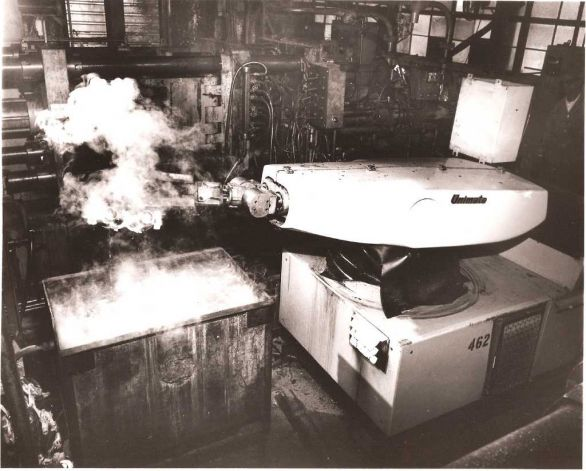
\includegraphics[width=.3\linewidth]{img/unimate}}
		\hspace{0.1cm}
		\subfloat[]{\label{fig:ancients}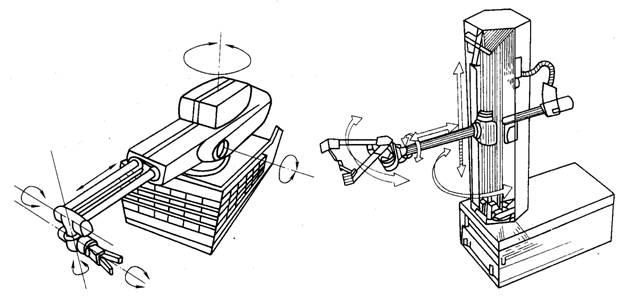
\includegraphics[width=.3\linewidth]{img/ancients_draw}}
		\hspace{0.1cm}
		\subfloat[]{\label{fig:versatran}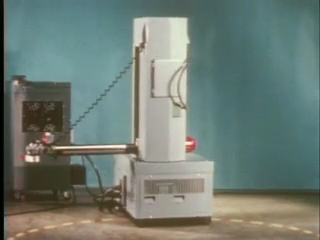
\includegraphics[width=.3\linewidth]{img/versatran}}
	\end{center}	
	\centering
	\captionsetup{justification=centering,margin=2.5cm}
	\caption{(a) Robot \textit{Unimate}, (b) esquemas del \textit{Versatran} y del \textit{Unimate} y (c) Robot \textit{Versatran}.}
	\label{fig:robots1}
\end{figure}

Este primer desarrollo marcó un hito que inició una carrera masiva de diversos tipos de robots para todo tipo de tareas. En los años sucesivos, debido al crecimiento del sector industrial, la robótica se centró principalmente en los entornos más industrializados. De este crecimiento comenzaron a aparecer robots que se ocupaban de la automatización de las tareas más peligrosas, aburridas e incluso tareas que requerían de gran precisión. Esto supuso que cada vez más, los humanos fueran centrándose en otro tipo de tareas a más alto nivel como la investigación y desarrollo de robots más sofisticados. Un ejemplo importante de la época en el sector industrial fue el robot \textit{Versatran} ((Figura \ref{fig:versatran}), desarrollado para transportar cargas dentro de la fábrica de ensamblaje de automóviles Ford, en 1962.

En 1969 aparecen los primeros robots soldadores tan utilizados hoy en día en cadenas de montaje. Este tipo de robots surge de la falta de precisión y velocidad de los trabajadores humanos a la hora de realizar soldaduras a los vehículos en las cadenas de producción. Estos robots supusieron mejoras importantes en las condiciones de los trabajadores, ya que el trabajo de soldadura era considerado como peligroso y dañino para las personas. Además, las cadenas de montaje también se vieron beneficiadas ya que estos robots, al ser muy precisos y veloces en las soldaduras, aumentaron en gran medida la productividad de las fábricas; tarea que un humano no podía llevar a cabo de forma tan rápida, segura y fiable.

A lo largo de los años y gracias a los avances en investigación, los robots han ido mejorando paulatinamente en cuanto a desempeño de tareas cada vez más complejas. Hoy en día existen robots capaces de llevar a cabo tareas complejas no sólo en el campo de la investigación, sino en el ámbito doméstico o industrial. Como se ha comentado, los robots son ideales para realizar tareas repetitivas, peligrosas o aburridas para las personas. Aparte de la ya mencionada tarea de soldadura, el ámbito industrial se ha visto beneficiado en las cadenas de producción y en tareas logísticas, por ejemplo, con los robots utilizados para el embalaje de magdalenas (Figura \ref{fig:cupcake_robot}), robots para levantar cargas pesadas de forma autónoma, transporte de herramientas, y multitud de propósitos diferentes. Uno de los ejemplos más claros en la automatización del sector industrial es \textit{Amazon}. Esta empresa cuenta con una flota de robots autónomos que se encargan de transportar mercancías dentro de sus naves industriales \footnote{\url{https://www.youtube.com/watch?v=tMpsMt7ETi8}}. para agilizar la logística de paquetes. Debido a la creciente demanda de transportes más rápidos con el auge de las compras por internet (\textit{e-commerce}) es crucial que la logística sea lo más rápida, precisa y robusta posible, lo que \textit{Amazon} consigue con el uso de robots completamente autónomos que puedan operar las 24 horas del día.

\begin{figure}
	\begin{center}
		\subfloat[]{\label{fig:beast}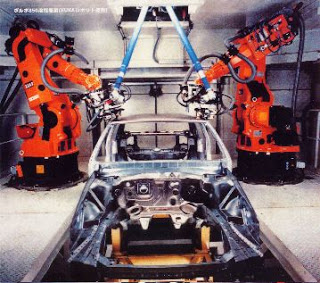
\includegraphics[width=.33\linewidth]{img/beast}}
		\hspace{0.1cm}
		\subfloat[]{\label{fig:stanford_cart}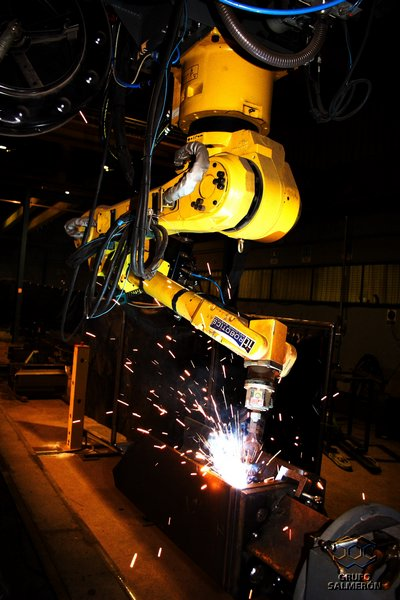
\includegraphics[width=.3\linewidth]{img/stanford_cart}}
	\end{center}	
	\centering
	\captionsetup{justification=centering,margin=0.1cm}
	\caption{(a) y (b) robots soldadores en plantas de producción industrial.}
	\label{fig:robots2}
\end{figure}

Del auge de la robótica no solamente se ha visto beneficiado el sector industrial. Otro foco en el que cada vez se centran más las empresas es la robótica en el ámbito doméstico. Actualmente, en este sector se comercializan diferentes tipos de robots que resultan muy útiles en las tareas del hogar. Un claro ejemplo son los robots aspiradores; empresas como iRobot con el \textit{Roomba} (Figura \ref{fig:roomba}) o Xiaomi con su \textit{Mi Robot Vacuum} (Figura \ref{fig:xiaomi}) son pioneras en este sector.

\begin{figure}
	\begin{center}
		\subfloat[]{\label{fig:cupcake_robot}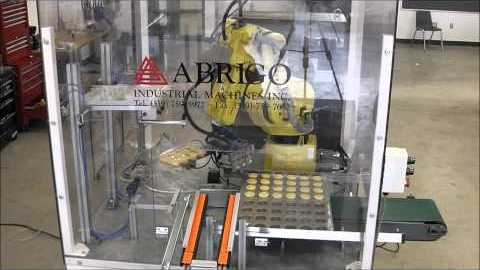
\includegraphics[width=.34\linewidth]{img/cupcake_robot}}
		\hspace{0.1cm}
		\subfloat[]{\label{fig:roomba}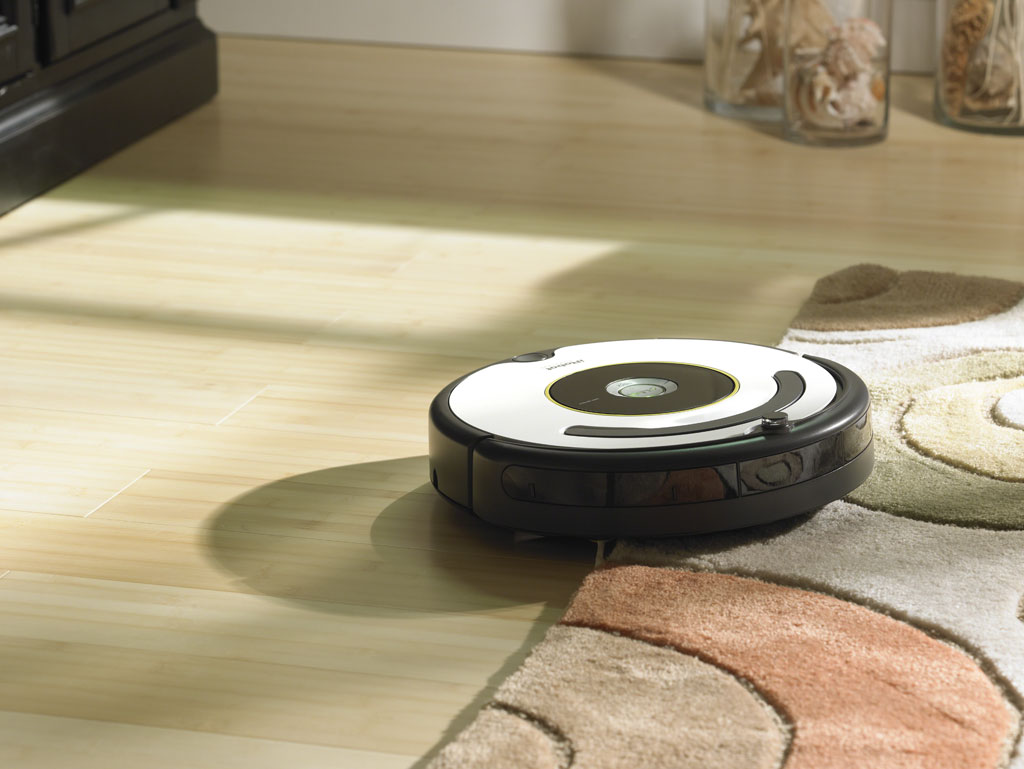
\includegraphics[width=.255\linewidth]{img/roomba}}
		\hspace{0.1cm}
		\subfloat[]{\label{fig:xiaomi}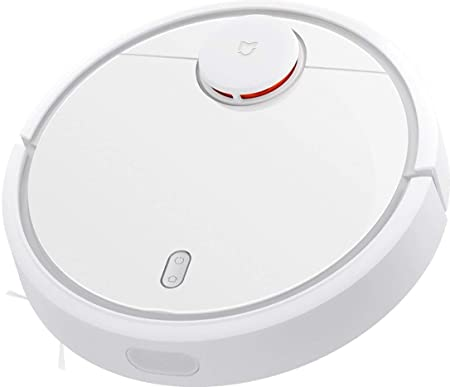
\includegraphics[width=.25\linewidth]{img/xiaomi}}
	\end{center}
	\centering
	\captionsetup{justification=centering,margin=2cm}
	\caption{(a) Robot embalador de magdalenas, (b) \textit{Roomba} de iRobot y (c) \textit{Mi Robot Vacuum} de Xiaomi.}
	\label{fig:robots3}
\end{figure}

Por último, cabe mencionar que en la actualidad, la conducción autónoma se ha puesto a la cabeza de los problemas a investigar por parte de las empresas y de la comunidad científica. La conducción autónoma trata de solucionar el problema de que un vehículo sea capaz de emular la capacidad de un humano de conducir tomando como información la proporcionada por diferentes sensores como cámaras (RGB, RGBD, monocromáticas, etc.), láser, radar, etc. El problema es complejo, ya que no sólo es necesario que el vehículo sea capaz de mantenerse dentro de la carretera, sino que además deberá cumplir con todas las normas de circulación pertinentes al igual que debe hacer un humano, además de ser capaz de tomar decisiones en multitud de escenarios y condiciones (baja visibilidad, cruce de peatones, accidentes, etc.) que se presentan durante la conducción. Es por esta complejidad que el problema aún no está resuelto.

Existe un estándar: el J3016, ideado por la SAE (Sociedad de Ingenieros automotrices) que categoriza los niveles de conducción autónoma de un sistema en base a las capacidades del vehículo. En la Figura \ref{fig:levelsdriving} se observa la taxonomía que hace referencia a los siguientes niveles:

\begin{enumerate}
    \item Nivel 0. No hay automatización; conduce un humano.
    \item Nivel 1. Asistencia al conductor. Algún sistema de apoyo como velocidad de crucero o auto aparcamiento. Sólo asiste al movimiento longitudinal o lateral.
    \item Nivel 2. Automatización parcial. El sistema puede tomar el control del vehículo en determinadas circunstancias controladas. No obstante el humano ha de supervisar en todo momento.
    \item Nivel 3. Automatización condicional. El sistema puede tomar decisiones en la conducción recibiendo información del entorno y calculando riesgos. El humano ha de intervenir cuando el sistema lo requiera.
    \item Nivel 4. Autonomía. El sistema tiene el control del vehículo; es capaz de detectar objetos y eventos y actuar ante ellos. 
    \item Nivel 5. Autonomía completa. No se requiere supervisión del humano; el sistema es capaz de realizar una conducción del vehículo en cualquier situación.
\end{enumerate}

\begin{figure}
  \centering
  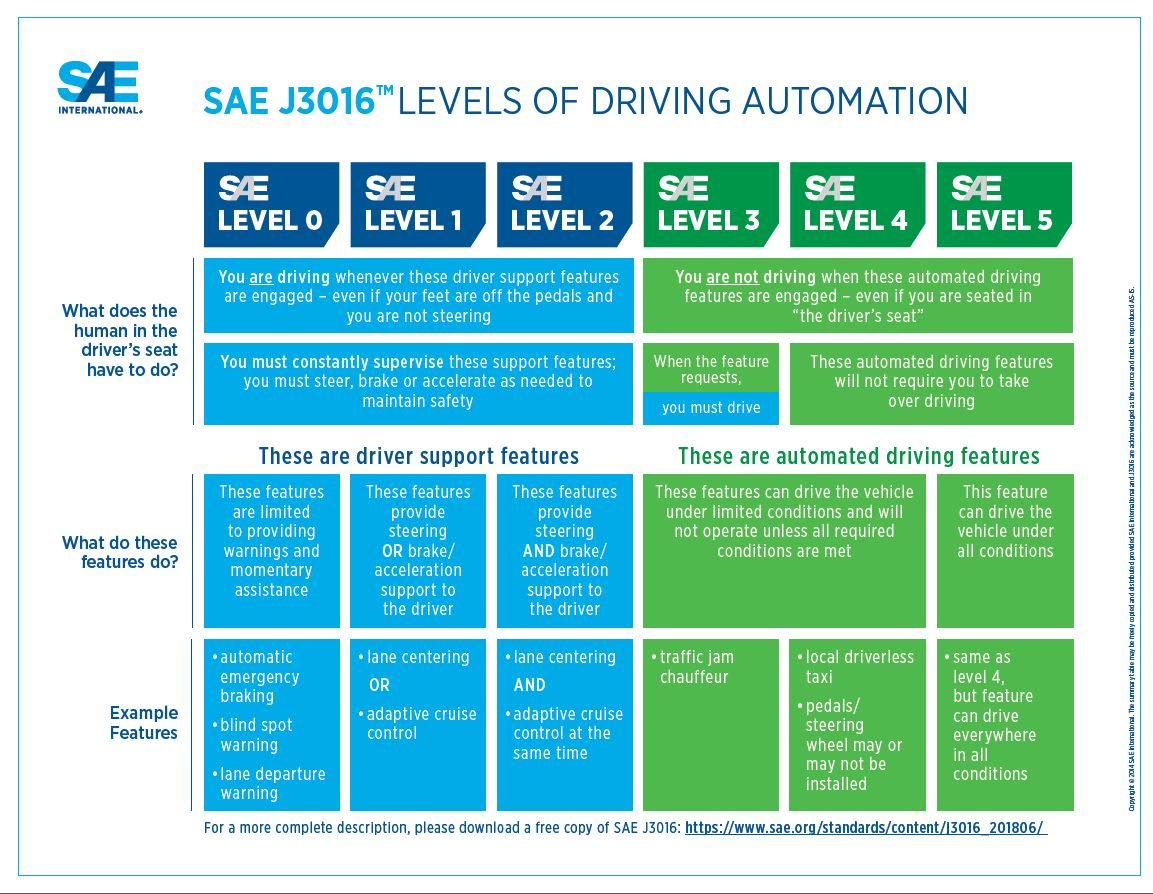
\includegraphics[width=.9\linewidth]{img/levels-of-driving}
  \caption{Niveles de conducción autónoma según el SAE}
  \label{fig:levelsdriving}
\end{figure}

Una de las empresas pionera en ofrecer soluciones a este problema de forma comercial es Tesla \footnote{\url{https://www.tesla.com}}, la cual desde hace ya algunos años comercializa vehículos con la tecnología necesaria para circular por una vía de forma autónoma, a la que han bautizado como \textit{AutoPilot}. No obstante, la empresa ofrece esta tecnología como un <<asistente para la conducción>> ya que, a pesar de que se ha demostrado que el coche es capaz de realizar la tarea, aún necesita la supervisión constante de un humano para evitar accidentes. Teniendo en cuenta la lista del SAE, se puede ver que la tecnología de Tesla está aún en el nivel 2, lo cual dista mucho aún de la conducción autónoma total.

El nivel más alto de esta lista lo tiene Google, con su proyecto Waymo. Teóricamente, Waymo está actualmente en el nivel 4 de la lista de SAE, aunque aún está en etapa de investigación. La tecnología de Waymo ha sido probada con éxito en diferentes entornos tanto de ciudad como de carretera de forma exitosa, no obstante, todas estas pruebas ha sido en entornos más o menos controlados. Este proyecto se explica con más detalle en la sección \ref{sec:robolearnvision}

En las siguientes secciones se explicará cómo conecta el problema de la conducción autónoma con la robótica, la visión artificial y el aprendizaje profundo, que son las tecnologías que enmarcan este proyecto.

\section{\textit{Deep Learning}}

El \textit{Deep Learning} o aprendizaje profundo es un campo dentro del aprendizaje automático (\textit{Machine Learning}) que utiliza estructuras de redes neuronales organizadas en capas para conseguir aprender representaciones de los datos más significativas conforme se avanza en las capas de la red. La palabra \textit{deep} hace referencia al número de capas que se utilizan en la red, por lo que se suele considerar que una red neuronal de más de 3 capas ya es una red neuronal profunda.

Una red neuronal es un tipo de estructura de cómputo que se caracteriza por emular el funcionamiento de un sistema nervioso humano, donde las diferentes neuronas conectadas entre sí trabajan juntas para solucionar un problema dentro de un dominio. La definición formal de una red neuronal es que es una función de aproximación de funciones universal, donde dado una serie de datos que entran a un sistema se pueda obtener una determinada salida deseada.

En la Figura \ref{fig:simplenet} se ilustra una arquitectura de red neuronal básica, conocida como perceptrón multicapa (MLP o \textit{MultiLayer Perceptron} por sus siglas en inglés). Esta red en particular consta de 3 capas: una capa de entrada, una capa oculta y una capa de salida. En la capa de entrada se representan los datos que ya han sido preparados para alimentar a la red en un formato determinado; la capa oculta se encarga, principalmente, de procesar la entrada de datos realizando los cálculos pertinentes para obtener una salida deseada utilizando los parámetros (pesos) de la misma; y en la capa de salida se reciben los datos procesados por la red neuronal. Todas las neuronas en una capa están conectadas con alguna (o todas) las neuronas de la capa siguiente, y a cada neurona se le asigna un número llamado peso que se utilizan como moduladores de la red. El proceso de aprendizaje consiste principalmente en ajustar esos pesos para que la red sea capaz de aprender a procesar los datos de entrada de manera que la salida sea igual o muy similar a la que se espera. Ese ajuste de pesos se realiza mediante ensayo-error de la siguiente manera: dada una entrada de datos $X=\{x_1,x_2,...,x_n\}$, la red procesará dichos datos y generará una salida estimada $\hat y$ que será comparada con la salida esperada $y$ produciendo un error (mediante alguna función como error cuadrático medio - MSE - o error absoluto medio - MAE -), ya que la salida de la red puede que no coincida exactamente con la salida esperada; el objetivo del aprendizaje de una red neuronal es que ese error se reduzca al máximo posible (idealmente el error será cero al final del entrenamiento, ya que la salida de la red y la salida esperada serán la misma, es decir, la red no ha cometido errores); para ello, cada vez que la red procesa una muestra de datos ésta actualiza sus pesos mediante una técnica llamada \textit{back propagation}, que recibe su nombre por la forma en que el error cometido por la red se propaga hacia atrás actualizando los pesos de todas (o algunas) sus capas mediante cálculos de derivadas. 

\begin{figure}
  \centering
  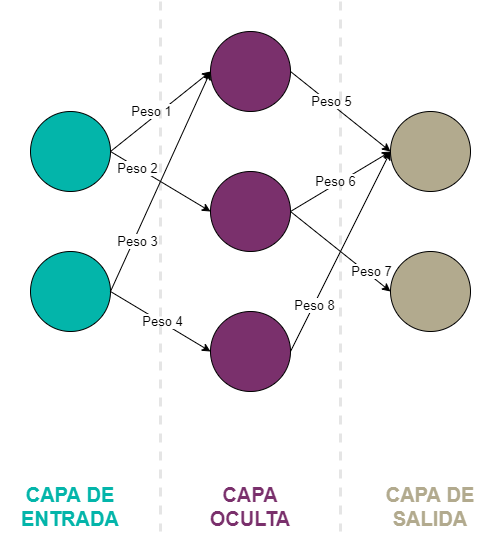
\includegraphics[width=.6\linewidth]{img/simplenet}
  \caption{Esquema de red neuronal sencilla}
  \label{fig:simplenet}
\end{figure}

Las redes neuronales pueden tener multitud de formas diferentes, con distintas configuraciones en cuanto a número de capas, número de neuronas por capa, conexiones entre neuronas, etc. Actualmente, los modelos más grandes diseñados para tareas tanto de visión artificial como de procesamiento de lenguaje natural (NLP), que son dos de los campos donde el aprendizaje profundo ha tenido más impacto en la última década, pueden tener cientos de capas. No obstante, los primeros modelos neuronales eran mucho más pequeños debido a la limitación en la capacidad de cómputo.

En 2006 Geoffrey Hinton \cite{geoffreyhinton} propone un nuevo método de entrenamiento de las redes neuronales existentes hasta el momento, utilizando un entrenamiento por capas; de esta forma, cada capa de la red irá aprendiendo diferentes características de los datos de entrada empezando por las características más primitivas hasta las características más complejas extraídas de los datos según se avanza en las capas de la red. Este procedimiento se lleva a cabo hasta que se han entrenado todas las capas de la red. Este avance permitió el entrenamiento de redes mucho más profundas que las existentes en ese momento, popularizando el término \textit{deep learning} o aprendizaje profundo en castellano. Con el tiempo se ha demostrado que las redes neuronales más profundas otorgan resultados mucho mejores que otros modelos con menos capas o que las técnicas clásicas de \textit{machine learning}.

En 2012, se inicia una revolución en el campo de la visión artificial con la llegada de AlexNet \cite{alexnet}. Alex Krizhevsky batió todos los récords de precisión en el problema de clasificación de imágenes en el torneo anual de \textit{ImageNet} en 2012 al proponer un modelo basado en aprendizaje profundo con redes neuronales convolucionales acelerando el cómputo a través de GPU. Después de competir en el \textit{ImageNet Large Scale Visual Recognition Challenge} \footnote{http://image-net.org/challenges/LSVRC/}, AlexNet saltó a la fama. Logró un error del 15,3\%. en la tarea de clasificación de imágenes, que fue un 10,8\% más bajo que el del segundo puesto. Este resultado fue gracias a la profundidad del modelo que era necesaria para su alto rendimiento y al uso de las redes neuronales convolucionales (CNN). En 2012 este tipo de procesamiento era muy caro desde el punto de vista computacional, pero se hizo factible gracias al uso de las GPU (\textit{Graphic Processing Unit} o Unidades de procesamiento gráfico) durante el entrenamiento.
Tras este hito, el campo de la visión artificial explotó y comenzaron a surgir multitud de modelos novedosos que expandieron los límites del aprendizaje profundo mejorando las técnicas de aprendizaje automático que existían hasta el momento. Esta revolución dio pie a la resolución de diferentes tipos de problemas usando la visión artificial en campos como la industria (p.e.: detección de imperfecciones en cadenas de montaje), la robótica (p.e.: navegación autónoma), la medicina (p.e.: detección de cáncer de mama), etc.

Uno de los proyectos de visión aritificial más ambiciosos de la última década ha sido GoogleBrain, que surgió también en 2012 de la mano de Jeff Dean y de Andrew Ng. Para este proyecto se desarrolló una red neuronal profunda que era capaz de detectar patrones en imágenes y vídeos de Youtube, llegando a ser capaz de reconocer gatos en vídeos de Youtube analizando las imágenes de cada fotograma. Dos años más tarde, la empresa DeepMind, dedicada al mundo de los videojuegos y el \textit{deep learning}, es absorbida por Google. En 2016, DeepMind consiguió batir al mejor jugador del mundo (Lee Sedol) en el juego de mesa Go por 5 a 1, utilizando su algoritmo de \textit{deep learning}: AlphaGo, mediante jugadas <<creativas>> y <<nunca vistas>> según jugadores de Go profesionales. No obstante, un año después crearon AlphaGo Zero, que es igual de potente que el AlphaGo original, pero con la característica de que es un sistema autodidacta, esto es, que ha aprendido por sí mismo a jugar al juego mediante aprendizaje por refuerzo jugando contra sí misma sin ningún tipo de información a priori. AlphaGo y AlphaGo Zero se basan en la visión para procesar las jugadas en cada turno, y tomar decisiones en función de la disposición de las fichas en el tablero.

En la acutalidad la IA se encuentra en plena ebullición. Tanto es así que una gran mayoría de empresas tecnológicas quieren implementar soluciones basadas en el \textit{deep learning} para sus productos y/o servicios. Así, las grandes empresas tecnológicas como Google, Amazon, Facebook, Tesla, etc., ya ofrecen soluciones basadas en IA en diferentes campos como el NLP, la visión artificial o la robótica. Como ejemplos de los últimos dos años tenemos el algoritmo GPT-3 para generación automática de texto (creado por OpenAI); Google Home y Amazon Echo Dot (Figura \ref{fig:homeecho}) que son asitentes de voz inteligentes; Facebook utiliza el \textit{deep learning} para orientar sus anuncios e identificar objetos en las imágenes subidas por sus usuarios; Google con su buscador utiliza \textit{deep learning} con modelos basados en Transformers \cite{transformers} para obtener mejores resultados en las búsquedas, incluso Amazon en sus almacenes con su flota de robots logísticos que utilizan \textit{deep learning} para moverse de forma eficiente por las naves, y también Tesla y Google con sus proyectos de conducción autónoma basados en IA Autopilot\footnote{\url{https://www.tesla.com/autopilot}} y Waymo\footnote{\url{https://waymo.com}} respectivamente.

\begin{figure}
  \centering
  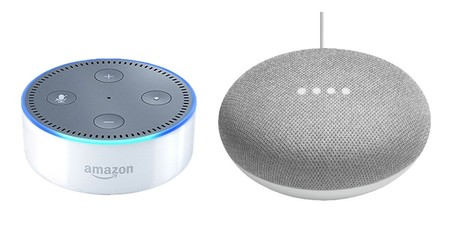
\includegraphics[width=.9\linewidth]{img/homeecho.jpg}
  \caption{Amazon Echo Dot y Google Home}
  \label{fig:homeecho}
\end{figure}


Una de las grandes compañías que han apostado por el \textit{deep learning} es Facebook. Con Yann LeCun a la cabeza en el laboratorio de IA de Facebook, se desarrolla DeepFace \cite{deepface} en 2014. DeepFace es un algoritmo basado en \textit{deep learning} que es capaz de reconocer rostros en imágenes digitales con la misma precisión que un humano.

Una empresa de nacimiento reciente que es consecuencia de la explosión en la IA es OpenAI\footnote{\url{https://openai.com}}. Esta empresa fundada por el dueño de empresas como Tesla y SpaceX, Elon Musk, se dedica a la investigación sobre diferentes campos de la IA sin ánimo de lucro. Uno de sus mayores logros desde su fundación es la creación de sus modelos de generación de texto en lenguaje natural: GPT-2 y su actual versión GPT-3. Estos dos modelos utilizan arquitecturas Transformers (que provocaron la explosión del campo del procesamiento del lenguaje natural o NLP en 2018), que son modelos de redes neuronales mucho más potentes que las LSTM permitiendo obtener información contextual con mucho mayor alcance temporal. Los algoritmos GPT-2 y GPT-3 tienen como objetivo la generación de texto en lenguaje natural simulando a un humano. Es tal la potencia de dichos modelos, que a pesar de que OpenAI es una empresa de \textit{softwre} libre, no liberaron el modelo de GPT-2 por el peligro que suponía en la generación de noticias falsas o textos de odio de forma masiva. A día de hoy, y como ya sucedió en 2012 con el campo de la visión artificial, el NLP está en pleno auge; incluso Google implementa modelos basados en estas arquitecturas para su buscador.

\section{\textit{Deep Learning} aplicado a la robótica con visión}
\label{sec:robolearnvision}

Uno de los campos de la ingeniería que mejor casa con el aprendizaje profundo es la robótica. Esto es así porque la <<inteligencia>> que se asocia a los robots se basa en su autonomía, es decir, la capacidad del robot de llevar a cabo comportamientos simples o complejos de forma totalmente autónoma. Históricamente estos comportamientos complejos se lograban mediante algoritmos sofisticados con mucha lógica de control, lo que llevaba a hacer que los algoritmos que generaban estos comportamientos fueran muy complejos y con una casuística muy extensa. Con la explosión del \textit{deep learning} el campo de la robótica se ha visto enormemente beneficiado, ya que la algoritmia subyacente que conseguía la autonomía de los robots se ha simplificado en gran medida al añadir el factor de aprendizaje. Uno de los campos que más impacto ha tenido sobre la robótica aplicando el aprendizaje profundo ha sido la visión artificial. Actualmente la visión artificial aplicada a robots se puede ver en multitud de proyectos muy novedosos y en auge como la conducción autónoma con Tesla y Google a la cabeza (Figura \ref{fig:cameras}); en el ámbito industrial con las cadenas de producción (robots soldadores, robots ensambladores, etc.); en el ámbito doméstico con las aspiradoras robóticas con cámara integrada que implementan algoritmos de SLAM visual (\textit{Simultaneous Localization and Mapping} por sus siglas en inglés); y sobretodo en el ámbito de la investigación, donde hay multitud de estudios en curso sobre la visión artificial aplicada a la robótica.

\begin{figure}
	\begin{center}
		\subfloat[]{\label{fig:cupcake_robot}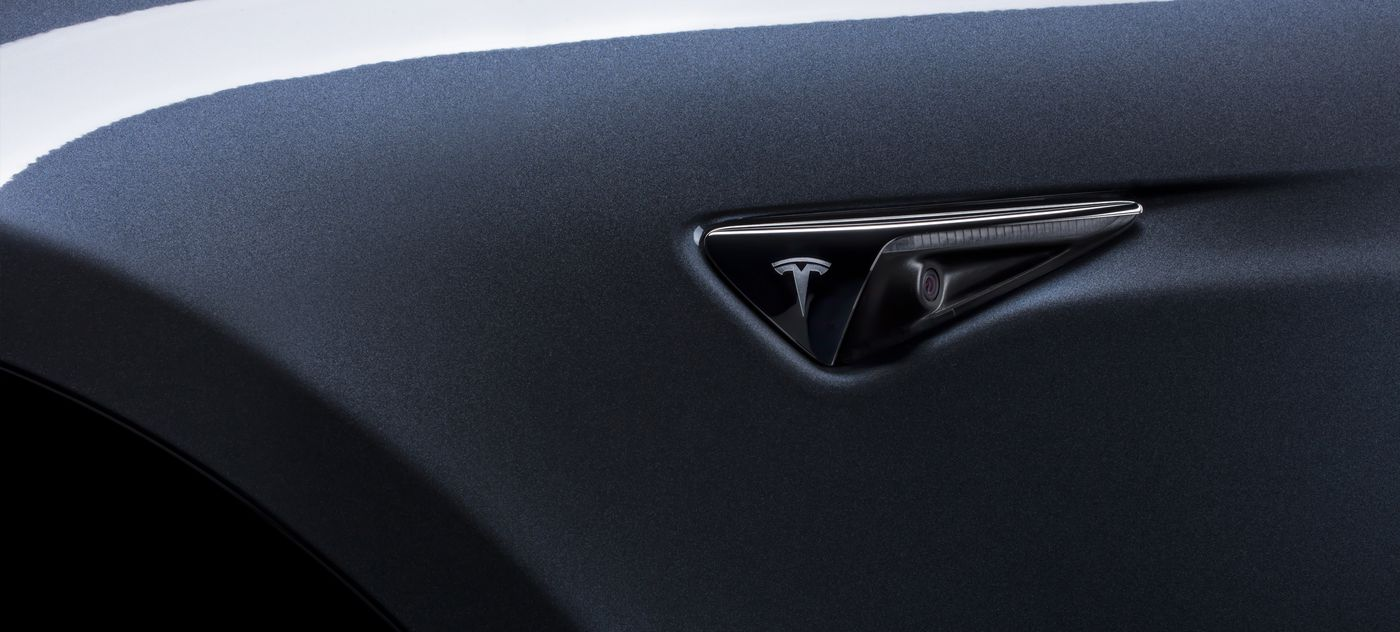
\includegraphics[width=.50\linewidth]{img/teslacam.jpg}}
		\hspace{0.1cm}
		\subfloat[]{\label{fig:roomba}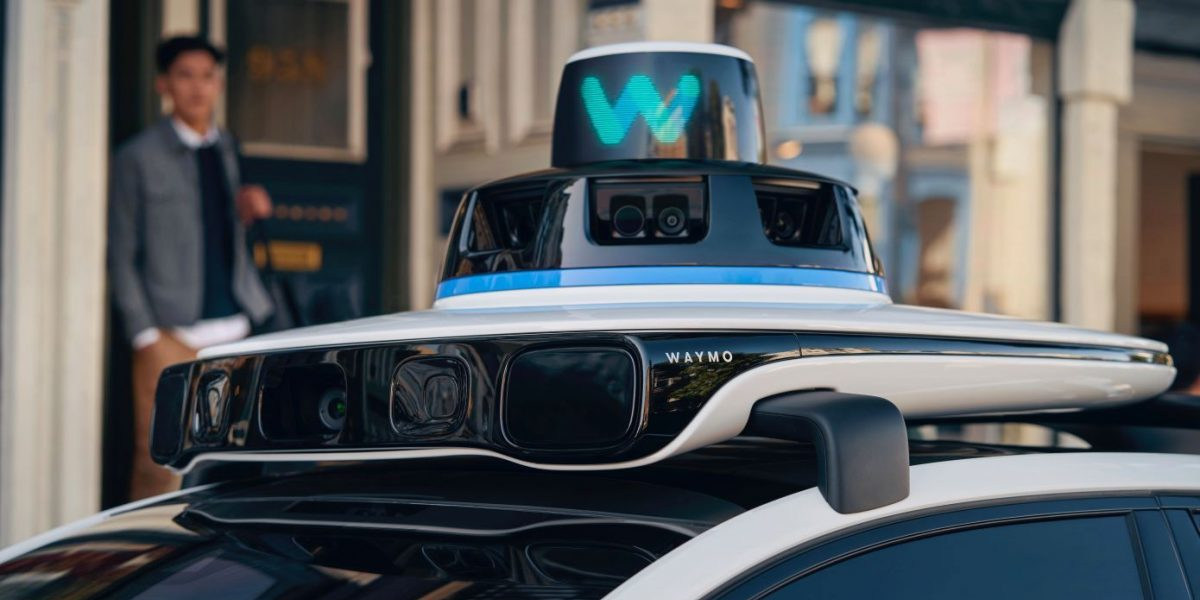
\includegraphics[width=.45\linewidth]{img/waymocam.jpg}}
	\end{center}
	\centering
	\captionsetup{justification=centering,margin=2cm}
	\caption{(a) Cámara del \textit{AutoPilot} del Tesla, (b) Cámaras del coche Waymo de Google.}
	\label{fig:cameras}
\end{figure}


Un ejemplo perfecto de la visión aplicada a la robótica en línea con este proyecto es el ya mencionado Waymo, de Google. El proyecto Waymo comenzó en 2009 y su objetivo principal es el de resolver la tarea de la conducción autónoma. Como se comentó en anteriores secciones, el nivel de autonomía máxima de la conducción autónoma es el nivel 5; Waymo ya ha conseguido llegar al nivel 4. Google se centra sobretodo en la conducción en entornos urbanos, donde, a priori, el problema es más complejo por el nivel de variables y situaciones imprevistas que pueden presentarse durante la conducción y a las que los conductores humanos se enfrentan todos los días. Este proyecto lo han bautizado como Waymo One\footnote{\url{https://waymo.com/waymo-one/}}. Adicionalmente, Google tiene además un proyecto paralelo para conducción de vehículos de logística (furgonetas de reparto y camiones de transportes de mercancías) llamado Waymo Via\footnote{\url{https://waymo.com/waymo-via/}}, más orientados a profesionales del transporte logístico. En la figura \ref{fig:waymo} se pueden ver algunos vehículos utilizados en ambos proyectos.

Waymo One lleva 3 años operando en Phoenix (Arizona) de forma comercial como servicio de taxis autónomos. Las pruebas realizadas por Waymo One están limitadas a un área metropolitana de esta ciudad, restringiendo su zona de actuación a dichas áreas. Este servicio de taxis autónomos opera a través de una aplicación con la que los usuarios pueden contratar un servicio de taxi como cualquier otro. Todos los taxis de Waymo operan con modelos Chrysler Pacifica modificados con todos los sensores necesarios para la conducción autónoma; no obstante, todos los taxis están supervisados en todo momento por un conductor humano que estará listo para intervenir cuando la situación lo requiera. 

Los vehículos autónomos de Waymo están diseñados para tener autonomía completa con sensores que otorgan visión en los 360 grados y láseres con alcance máximo de 300 metros de distancia. Entre los sensores integrados en los vehículos se encuentran: cámaras para la detección de carriles, láseres de corto alcance para detección de objetos cercanos, radar para la monitorización de objetos en movimiento (otros vehículos, peatones, etc.). Además integra interfaces en el interior del vehículo para que los supervisores humanos puedan interactuar con las funciones que ofrece el sistema. Para las pruebas, los ingenieros de Google crearon un simulador llamado Carcraft, que simula las diferentes condiciones de conducción con 25,000 coches virtuales autónomos en las calles de Texas, Mountain View y Phoenix.

\begin{figure}
  \centering
  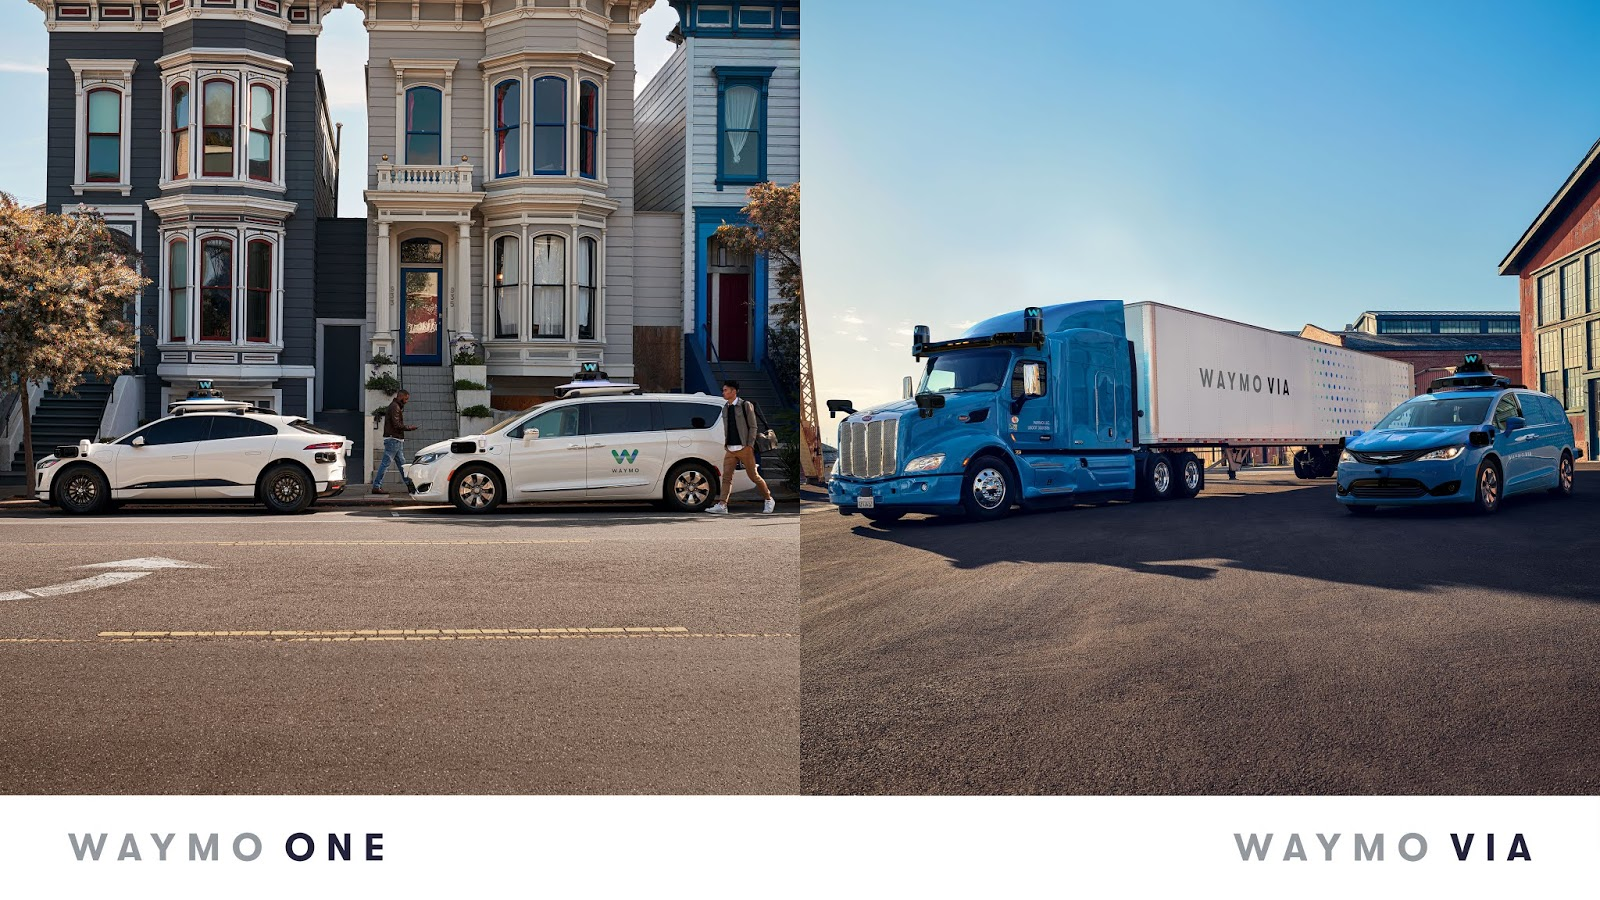
\includegraphics[width=.9\linewidth]{img/waymo_one_via.jpg}
  \caption{Proyectos en marcha de Google Waymo}
  \label{fig:waymo}
\end{figure}

A pesar de todos los avances conseguidos por Google, su sistema no es infalible, ya que se han registrado varios accidentes a lo largo de los años de vida del proyecto. Google sigue investigando en el problema de la conducción autónoma y ya ha conseguido llegar al nivel 4 del estándar de la SAE (Figura \ref{fig:levelsdriving}), sin ningún piloto al volante en algunos entornos controlados sin condiciones climáticas adversas, en carreteras con poca densidad de tráfico y sistemas de carreteras no complejos. Lo que indica que el problema aún no está resuelto del todo.

Por su parte, el proyecto Waymo Via sigue avanzando en investigación. Este proyecto comenzó su andadura en 2017 en las carreteras de California y Arizona.  Se estima que para 2020 esas rutas se amplíen a Texas y Nuevo México. También se engloban en Waymo Via los vehículos de reparto comerciales. Este año 2020 Google ha anunciado un programa piloto con la empresa de reparto UPS, donde los vehículos autónomos se encargarán de transportar la mercancía de las tiendas de UPS a una instalación logística de la misma empresa. Los camiones de transporte de mercancías y las furgonetas de reparto de Google incorporan la misma tecnología que los coches autónomos de Waymo One.

Por otra parte, en el ámbito de la investigación han surgido multitud de proyectos diferentes en la última década que relacionan estos tres campos: la robótica, la visión artificial y el aprendizaje profundo. Algunos de ellos se citan a continuación.

En \cite{deformable} se estudió la capacidad de las redes neuronales para reconocer objetos textiles que cuelgan de un sólo punto, como si una pinza robótica los estuviera cogiendo. Se probó con diferentes prendas como pantalones, toallas y camisas de colores, formas y materiales diversos. Con un conjunto de 6 prendas los autores consiguieron una precisión del 100\% prediciendo además el punto de agarre de la prenda con un error de aproximadamente 5 cm. Como estudio comparativo, demostraron que la aproximación basada en redes neuronales profundas de visión mejoraban a algoritmos clásicos como SVMs.

En \cite{tactile} se propone un estudio para solucionar el problema del agarre robótico. En este trabajo integraron la percepción visual y la percepción de contacto para realizar una clasificación háptica de los objetos (suave, rugoso, duro, pesado, etc.). Este sistema integrado en un robot podría predecir de antemano el tipo de objeto antes de entrar en contacto con él, para ajustar su agarre en función del objeto. Por ejemplo, un agarre de un objeto frágil como un huevo, necesita menos presión que un objeto más duro y pesado como una bola metálica.

En \cite{synergy} mediante el uso de una arquitectura de redes neuronales a la que llaman \textit{Visuo-Motor Deep Dynamic Neural Network}  (VMDNN) que es una arquitectura basada en redes neuronales recurrentes (RNN), consiguen enseñar a un robot a reconocer gestos hechos por un humano, a <<prestar atención>> y a la clasificación de objetos y el ajuste del agarre. En este estudio se hizo uso de un robot que observaba a un colaborador humano, en un escenario en el que había dos objetos diferentes. La tarea del humano era señalar a uno de los dos objetos para que el robot enfocara su atención en el objeto señalado, lo reconociera y ajustara el agarre para ese objeto determinado. El sistema logró un agarre satisfactorio un 85\% de las veces en simulación, utilizando el simulador iCub.

Por último, en \cite{manuver} entrenaron un modelo neuronal basado en redes neuronales recurrentes RNN para predecir las maniobras de tráfico en un vehículo conducido por un humano. El objetivo del trabajo era mejorar los sistemas anti colisión implantados en los coches autónomos, que típicamente no reaccionan a tiempo para evitar un accidente. Se entrenó este modelo en aproximadamente 1900 kilómetros de carreteras de alta y baja velocidad con 10 conductores diferentes. Los datos de entrenamiento incluían el vídeo desde la posición del conductor, el vídeo de la carretera frente al vehículo, la dinámica del vehículo, las coordenadas GPS y los mapas de las calles alrededor de la posición del vehículo.

\section{Objetivos}

Una vez presentado el contexto en el que se desarrolla este trabajo, a continuación se plantea y describe el problema abordado, así como la metodología aplicada al desarrollo \textit{software} de las soluciones propuestas.

El objetivo principal de este trabajo es conseguir un algoritmo de control visual para conducción autónoma basado en \textit{deep learning} y aplicar la solución a un robot pequeño en un entorno real. Además, se propone el desarrollo de una plataforma \textit{software} para la ejecución de comportamientos neuronales orientado a la conducción autónoma bautizada como BehaviorStudio\footnote{\url{https://jderobot.github.io/BehaviorStudio/}}, que servirá como infraestructura para probar la solución aportada para el objetivo principal.

Para desarrollar este trabajo se han dividido ambos objetivos generales en subobjetivos más abordables para una mejor gestión del tiempo y una planificación más eficiente. Los puntos 3 y 4 están relacionados con el desarrollo de la plataforma BehaviorStudio, los puntos 5 y 6 con el desarrollo de la solución para la conducción autónoma, y los puntos 1, 2, 7 y 8 son comunes para ambos objetivos. Se detallan a continuación:

\begin{enumerate}
    \item Estudiar el estado del arte de redes neuronales, visión artificial y conducción autónoma para obtener una visión panorámica del problema a resolver y ayudar en la toma de decisiones para de proyecto.
    \item Estudiar el contexto previo a este proyecto mediante la lectura y la réplica del Trabajo de Fin de Máster de Vanessa Fernández \cite{vanessa}, trabajo del que parte este mismo ampliando una de sus líneas futuras.
    \item Diseño de la plataforma BehaviorStudio, generando todos los diagramas y documentación pertinente para el desarrollo del \textit{software}. En esta etapa se generarán los diagramas UML del diseño, \textit{mockups} de la aplicación y los requisitos de la misma.
    \item Desarrollo de los diferentes componentes de la plataforma BehaviorStudio, generación de pruebas unitarias y confirmación del funcionamiento en entornos simulados mediante validación experimental.
    \item Adquisición y montaje del robot escogido como plataforma \textit{hardware} para la resolución del objetivo principal. Instalación de todas las herramientas necesarias para el desarrollo. Pruebas de ensamblaje, teleoperación, conectividad y movilidad del robot. 
    \item Desarrollo de los algoritmos de control visual basado en \textit{deep learning} centrado en el uso de redes neuronales convolucionales para el problema de regresión utilizando redes recurrentes y aplicación de los mismos en el robot real.
    \item Integración de la solución para la conducción autónoma en la plataforma BehaviorStudio y pruebas para comprobar el correcto funcionamiento de todas las partes en un entorno real.
    \item Experimentación y evaluación de la solución conseguida sobre diferentes circuitos reales.
    
\end{enumerate}

\noindent Además de los subobjetivos arriba listados, se querrá satisfacer una serie de requisitos para considerar válido el desarrollo del proyecto. Estos requisitos son:

\begin{itemize}
    \item La plataforma BehaviorStudio deberá ofrecer un interfaz de usuario sencillo, intuitivo y usable. Además deberá ofrecer la posibilidad de mostrar la información sensorial en tiempo real.
    \item El robot deberá ser capaz de completar al menos una vuelta en cada circuito propuesto tanto en sentido horario como en sentido antihorario.
    \item La plataforma BehaviorStudio deberá funcionar indistintamente en entornos simulados y en reales.
    \item El proyecto al completo se desarrollará en Python utilizando las librerías de programación más novedosas como PyTorch y PyQt.
    \item Los algoritmos propuestos han de ser ágiles no tardando demasiado tiempo entre iteraciones para que el comportamiento de los robots sea reactivo y los movimientos más fluidos.
    \item Se utilizará el \textit{middleware} robótico ROS por la compatibilidad entre entornos reales y simulados y porque facilita las comunicaciones entre los diferentes componentes de la aplicación.
\end{itemize}

\section{Metodología}

Para la realización de este proyecto se ha optado por seguir un modelo de desarrollo en espiral (Figura \ref{fig:espiral}) basado en prototipos, ya que los objetivos de este proyecto se ajustan más a este tipo de metodología. El modelo en espiral se basa en la idea fundamental de abordar las tareas iterativamente de forma que en cada iteración se aumenta la complejidad del proyecto, permitiendo la generación de prototipos funcionales al final de cada una. Debido a que se esperaban cambios en los requisitos constantemente típicos en proyectos de investigación, se ha optado por este modelo que permite libertad a la hora de reajustar funcionalidades específicas en cada ciclo, además de hacer el proyecto escalable tanto en funcionalidad como en complejidad.

El modelo en espiral se realiza por ciclos o iteraciones que corresponden a las diferentes fases del proyecto software. Cada ciclo se compone de cuatro fases principales, en las que se realizan diferentes tareas:

\begin{itemize}
    \item \textbf{Determinar los objetivos}. Se definen las necesidades que debe cumplir el \textit{software} a desarrollar en cada iteración, contemplando los objetivos finales. Esto hace que la complejidad del proyecto y el coste del ciclo avancen en función del tiempo.
    \item \textbf{Evaluar alternativas}. Se deben tener en cuenta las diferentes formas de llegar al objetivo proponiendo alternativas a los distintos elementos del proyecto. Además se deben considerar los riesgos que puedan existir e intentar reducirlos al máximo.
    \item \textbf{Desarrollar y verificar}. Teniendo en cuenta las alternativas propuestas en la fase anterior, se debe elegir la mejor de ellas y desarrollarla para llegar a los objetivos propuestos, para que finalmente el proyecto de ese desarrollo sea verificado con las pruebas pertinentes.
    \item \textbf{Planificar}. Con los resultados de las pruebas realizadas en la fase anterior, se ha de planificar la siguiente iteración revisando los posibles errores cometidos durante el ciclo actual y se comienza con un nuevo ciclo.
\end{itemize}

Todo esto sumando a la posibilidad de llevar un control por hitos al final de cada iteración además de las reuniones semanales con el tutor realizadas durante todo el proceso de desarrollo, hacen de este modelo el ideal en nuestro proyecto, dado que cada reunión ofrece realimentación para lo hecho hasta el momento teniendo así continuamente el proyecto bajo control.

Todo el código fuente generado para este proyecto se divide en dos repositorios de Github. El código de entrenamiento de los modelos está en el repositorio de RoboticsLabURJC\footnote{\url{https://github.com/RoboticsLabURJC/2017-tfm-francisco-perez}}, y el código de la plataforma BehaviorStudio está en su propio repositorio\footnote{\url{https://github.com/jderobot/behaviorstudio}}

\begin{figure}
  \centering
  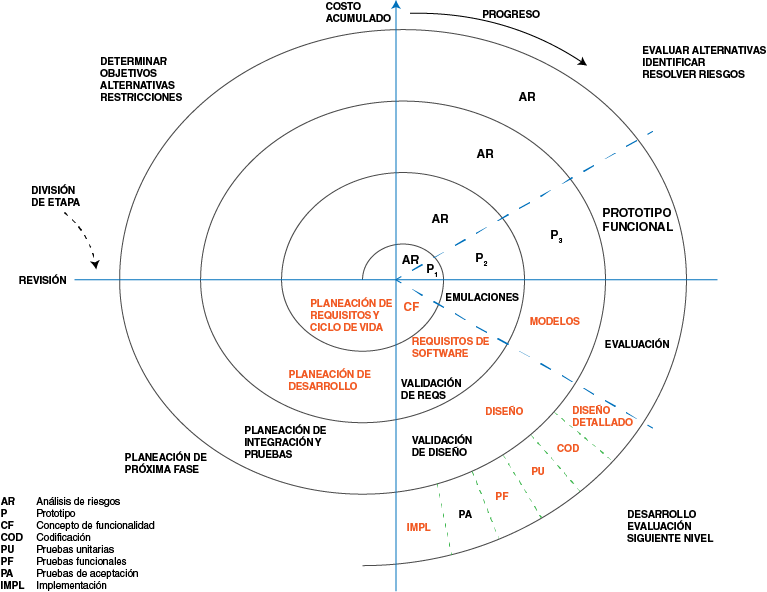
\includegraphics[width=.8\linewidth]{img/espiral.png}
  \caption{Metodología de desarrollo en espiral.}
  \label{fig:espiral}
\end{figure}
